\documentclass{article}
\usepackage{amsmath, amsfonts, amssymb, amsthm, stmaryrd}
\usepackage{enumitem}
\usepackage{hyperref}
\usepackage{bbm}
\usepackage{algorithm2e}

\usepackage[verbose=true,letterpaper]{geometry}
\newgeometry{
  textheight=9.5in,
  textwidth=6in,
  top=0.5in,
  headheight=12pt,
  headsep=25pt,
  footskip=30pt
}

%%%%%% Commands and theorems
\theoremstyle{plain}
\newtheorem{Theorem}{Theorem}
\newtheorem{Proposition}{Proposition}
\newtheorem{Corollary}{Corollary}
\newtheorem{Lemma}{Lemma}

\theoremstyle{remark}
\newtheorem{Definition}{Definition}
\newtheorem{Assumptions}{Assumptions}

\renewcommand{\P}{\mathbb{P}}
\newcommand{\E}{\mathbb{E}}
\newcommand{\R}{\mathbb{R}}
\newcommand{\N}{\mathbb{N}}

\newcommand{\sign}{\text{sign}}
\newcommand{\1}{\mathbbm{1}}

\newcommand{\argmin}{\arg\min}

\usepackage{color}
\usepackage{todonotes}
\newcommand{\todoT}[1]{\todo[inline,color=blue!40]{{\textbf{T:}~}#1}}


% To include the section number in the equation numbering:
\numberwithin{equation}{section}
\title{Adaptive stopping in Monte-Carlo evaluation for Deep RL}
\date{}
\begin{document}
\maketitle
\section{Description of the problem}
In Reinforcement Learning, we often use Monte-Carlo methods to evaluate the performances of an algorithm. In particular, if we denote $e(A)$ some evaluation of algorithm $A$), the global score of an algorithm by 
$$S(A)=\frac{1}{N}\sum_{i=1}^N e_i(A) $$
where $e_1(A), \dots,e_N(A)$ are the evaluation of the algorithm $A$ on $N$ different seeds (i.e. $e_1(A),\dots,e_N(A)$ are supposed i.i.d).

The goal of this article is to evaluate how high $N$ must be to have a good control on $S(A)$. In particular, when we compare two algorithms $A_1$ and $A_2$, how can we choose the value of $N$ that is large enough to compare $S(A_1)$ and $S(A_2)$? This is a trade-off between computational time and the need to assess correctly the scores of $A_1$ and $A_2$.

\section{Adaptive stopping using Group Sequential Testing}
\subsection{Group sequential testing}
\todoT{Explain why must be careful when doing GST and that we can't just do several tests. Maybe also motivate using the confidence interval approach from NIPS article.}

To choose $N$ adaptively, we propose to use group sequential testing (GST). GST are used in particular in clinical trials in which case an early stopping is desirable when comparing two drugs. We choose to use GST in particular and not sequential testing because the data are often naturally grouped due to the parallelization of the computation.

GST often suppose strong models on the data, in particular it is often supposed that the data are i.i.d. from a Gaussian distribution. This assumption is often not verified in the case of $e_i(A)$ being evaluations from a RL algorithm. In particular, the distribution of $e_i(A)$ often presents several modes and it can sometimes contain outliers. 

\todoT{Explain why several modes and give examples of distributions of DeepRL algos on classical environments. Ref https://arxiv.org/pdf/1806.08295.pdf on this also.}

The presence of several modes in the distributions of the evaluations and the difficulty to make any distributional assumption justify a non-parametric approach of the problem, but to further justify this approach we did a study of the effect of model misspecification on simulated data when using Gaussian GST algorithm. 




\subsection{Proposed algorithm}

The non-parametric GST that we propose is taken from ()\todo{cite} in which the authors use exact permutation tests on linear rank statistics applied to group sequential testing. This test has the advantage of being entirely non-parametric, exact and robust. On the other hand, if the sample-size is too large this test can be computationally exphensive and also there can be some bias because we compare the ranks and not the means of the distributions.



If we denote by $n$ the size of a group and by $K$ the maximum number of groups (see Algorith~\ref{alg:adastop}), then the complexity of Permutation GST algorithm is ${n \choose n/2}^K$, which is reasonable for example for $n,K\le 6$. For higher values of $n$ and $K$, we may want to use random permutations to make an approximation of the boundary used in the GST. 


\begin{algorithm}[h]
\SetAlgoLined
\SetKwInput{KwParameter}{Parameters}
\KwParameter{Algorithms $A_1,A_2$, environment $\mathcal{E}$, number of blocks $K \in \N^*$, size of a block $n$, level of the test $\alpha\in (0,1)$.}
Define $2nK$ different seeds $s_{1,1},\dots,s_{1,n},s_{2,1},\dots,s_{2,n}$.\\
\For{$t=1,\dots,K$}{
\For{$i=1,2$}{
Train aglorithm $A_i$ on environment $\mathcal{E}$ on seeds $s_{i,tn},\dots,s_{i,(t+1)n}$.\\
Collect evaluations $e_{tn}(A_i),\dots,e_{(t+1)n}(A_i)$.\\
Compute $S_t(A_i)=\frac{1}{nt}\sum_{j=1}^{nt}e_{j}(A_i)$.
}
Test  $H_0: S_t(A_1)=S_t(A_2)$ versus $H_1: S_t(A_1)\neq S_t(A_2)$ using GST Algorithm~\ref{alg:gst}.\\
If reject $H_0$, break the loop.
}
If the test was never rejected, return accept. Else return reject.
\caption{Adaptive Stopping.}\label{alg:adastop}
\end{algorithm}




\todoT{Give several other proposition of GST algorithms. For now, I put the ``naive'' permutation GST in a different section.}
\todoT{Explain the algorithm from the exact permutation GST article}
\todoT{Theoretical concerns : \\
- is this test most powerfull in some class of tests ?\\
- Can we show that if the distribution is well behaved, then we really compare the means of the distributions ? Even with rank test.\\
- Explain the empirical mean permutation test and finish explaining the rank permutation test.\\
- Also show some robustness properties like insensitivity to outliers as this would show that our algorithm also answers the concerns of the NIPS article ?\\
- Can we show that when using uniform permutation to approximate the test, we are still efficient ? How many random permutation should be used ?
}

\noindent\textbf{High level description of the algorithm.}\\
Let $x_j=(x_{1,j},\dots,x_{n, j})\in \{0,1\}^n $ be the vector of assignements at step $j$. $x_{i,j}$ is $0$ if the evaluation $i$ in the $j^{th}$ group is comming from Agent 1 and it is $0$ if the reward is comming from  Agent 2. In our setting, this means that $x_{i,j}=0$ if $i \le n/2$ and $x_{i,j}=1$ if $i > n/2$. 

Let $e_j =(e_{1,j},\dots,e_{n,j}) \in \R^n$ be the vector of evaluations observed at step $j$. 

Let
$r_{j}^{(i)}=(r_{1,j}^{(i)},\dots,r_{n,j}^{(i)}) \in \N^n $ be the vector of ranks of $e_j$ after $i$ groups have been evaluated.  $r_{l,j}^{(i)}$ is the rank of the $l^{th}$ evaluation in the $j^{th}$ group among all the evaluations in the $i$ first groups. The superscript $(i)$ is necessary as the ranking changes when we add more groups in the data.

Define for any $j\le i$
$$R_j^{(i)}=(r_1^{(i)}, \dots,r_{j}^{(i)})\in \N^{nj}.$$
We test the hypothesis $H_0:$``Agent 1 and Agent 2 have same evaluation'' against the alternative hypothesis $H_1:$``Agent1 and Agent2 have different evaluations''. More precisely, we use a sum-rank test (usually called the Wilcoxon rank sum statistic which is equivalent to Mann–Whitney U test) to test if the probability of $X$ (Agent 1) being greater than $Y$ (Agent 2) is equal to the probability of $Y$ being greater than $X$.

If $X_i=(x_1,\dot,x_i)\in \{0,1\}^{ni}$, we consider the linear rank test statistic
$$w_i=R_i^{(i)}X_i.$$
$w_i$ is in our case the sum of the ranks of the evaluations of Agent 2 after merging the evaluations on the first $i$ groups together.

The data are then summarized using the $w_i$'s. The group sequential test proceed is described in Algorithm \ref{alg:gst}.
\begin{algorithm}[h]
\SetAlgoLined
\For{$k=1,\dots,K$}{
Observe $x_k$ and $e_k$.\\
Compute $w_k$ from $x_k$ and $e_k$.\\
Compute $b_k^-, b_k^+$ boundary values.\\
\If{$w_k \ge b_k^+$ or $w_k \le b_k^-$}{
Reject $H_0$, break the loop and returns the answer
}
\Else{
If $k=K$ then accept $H_0$ otherwise continue.
}}
\caption{Rank statistic GST}\label{alg:gst}
\end{algorithm}

The values of $b_k^-$ and $b_k^+$ such that the overall level of the group sequential test is $1-\alpha$ are computed using permutation methods.

Define the boundary generating function $f_i$ by 
$$f_i(w_i)=\P\left(b_1^-\le W_1\le b_1^+, \dots, b_{i-1}^-\le W_{i-1}\le b_{i-1}^+, W_i = w_i  \right)$$
if we know how to compute $f_i$, it it then possible to find $b_i^-$ and $b_i^+$ such that 
$$\P\left(W_1 \notin (b_1^-, b_1^+) \right)=q_1 \le \alpha\left(\frac{1}{K} \right) $$
and for any $i$, we have 
$$q_{i-1}+\P\left(b_1^-\le W_1\le b_1^+, \dots, b_{i-1}^-\le W_{i-1}\le b_{i-1}^+, W_i  \notin(b_i^-, b_i^+) \right)=q_i \le \alpha\left(\frac{i}{K} \right).$$
where $\alpha(p)$ is the so-called level spending function, a parameter of the test, it must verify $\alpha(0)=0$, $\alpha(1)=\alpha$ and be non-decreasing.

The main computational burden of the algorithm is in computing $f_i(w_i)$, to compute $f_i$ we need to enumerate all the possible values $f_i(w_i)$ can take for the possible choices of affectation $X$, i.e. we must enumerate $\Gamma_1 \times \dots \times \Gamma_i$ where
$$\Gamma_j= \left\{x_j: \sum_{l=1}^{2n}x_{j,l} = n,\quad x_{j,l}\in \{0,1 \}\right\}.$$
one element of $\Gamma_1 \times \dots \times \Gamma_i$ is equivalent to the path in a graph. The graph of $\Gamma_j$ is composed of nodes labelled by a couple $(a,b)$ where $(a,b)$ implies that of the first $a$ samples, exactly $b$ have been assigned to Agent 2.
\begin{figure}[ht]
\begin{center}
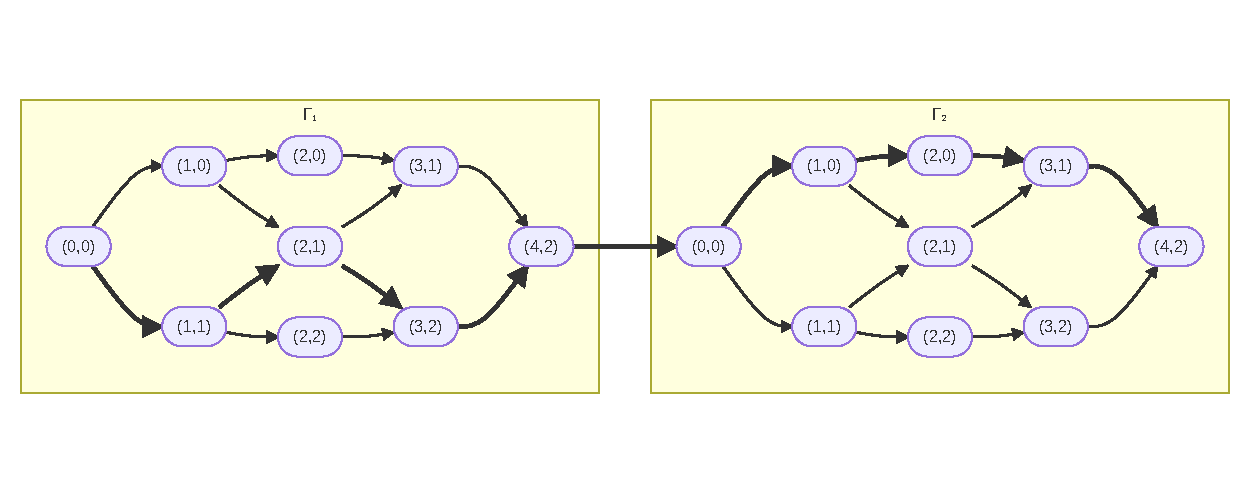
\includegraphics[scale=0.7]{graph_gamma.pdf}
\caption{Graph representation of $\Gamma_1$ and $\Gamma_2$. The thick path represent $x_i=(1,0,1,0,0,0,1,1)$}
\end{center}
\end{figure}


\newpage
\section{Simulation study}
\todoT{Misspecification study of Gaussian GST on uniform and maybe on multi-modal distributions}
\todoT{Comparison of GST algorithms on gaussian Data.}
\section{Experimental results}
\todoT{Apply to some classical algorithms on classical environments. Maybe also try to 
replicate adaptively the results of the NIPS article : do we also stop around 20 iterations when comparing two agents on an Atari environment? Or on the pybullets environments like in the article}
% \section{Other possible algorithms}
% \begin{algorithm}[h]
% \SetAlgoLined
% \SetKwInput{KwParameter}{Parameters}
% \KwParameter{Evaluations $e_1(A_i),\dots,e_t(A_i)$ for $i \in \{1,2\}$, level of the test $\alpha$, number of blocks $K$, number of permutations $B$.}
% Compute $t_0=S_t(A_1)-S_t(A_2)$.\\
% Define $Z_1,\dots,Z_{2t}$ with 
% $$Z_i = \begin{cases}e_i(A_1) & \text{ if }1\le i\le t\\ e_{i-t}(A) & \text{ if }t+1\le i\le 2t \end{cases} $$ 
% \For{$b=1,\dots,B$}{
% Draw a permutation $\sigma$ uniformly at random in $\mathcal{S}_{2t}$.\\
% Compute 
% $$t_b = \frac{1}{t}\sum_{i=1}^t Z_{\sigma(i)}-\frac{1}{t}\sum_{i=t+1}^{2t} Z_{\sigma(i)}$$
% }
% Let $q_1$ be the empirical quantile of level $\frac{\alpha}{2K}$ of $t_1,\dots,t_B$ and $q_2$ the empirical quantile of level $1-\frac{\alpha}{2K}$.\\
% If $t_0\le q_1$ or $t_0 \ge q_2$  then reject $H_0$. Else, do not reject $H_0$.
% \caption{Step $t$ of Union Bound Permutation GST.}\label{alg:gst}
% \end{algorithm}

\bibliographystyle{plain}
\bibliography{biblio_file}
\end{document}
